\begin{figure}
\centering
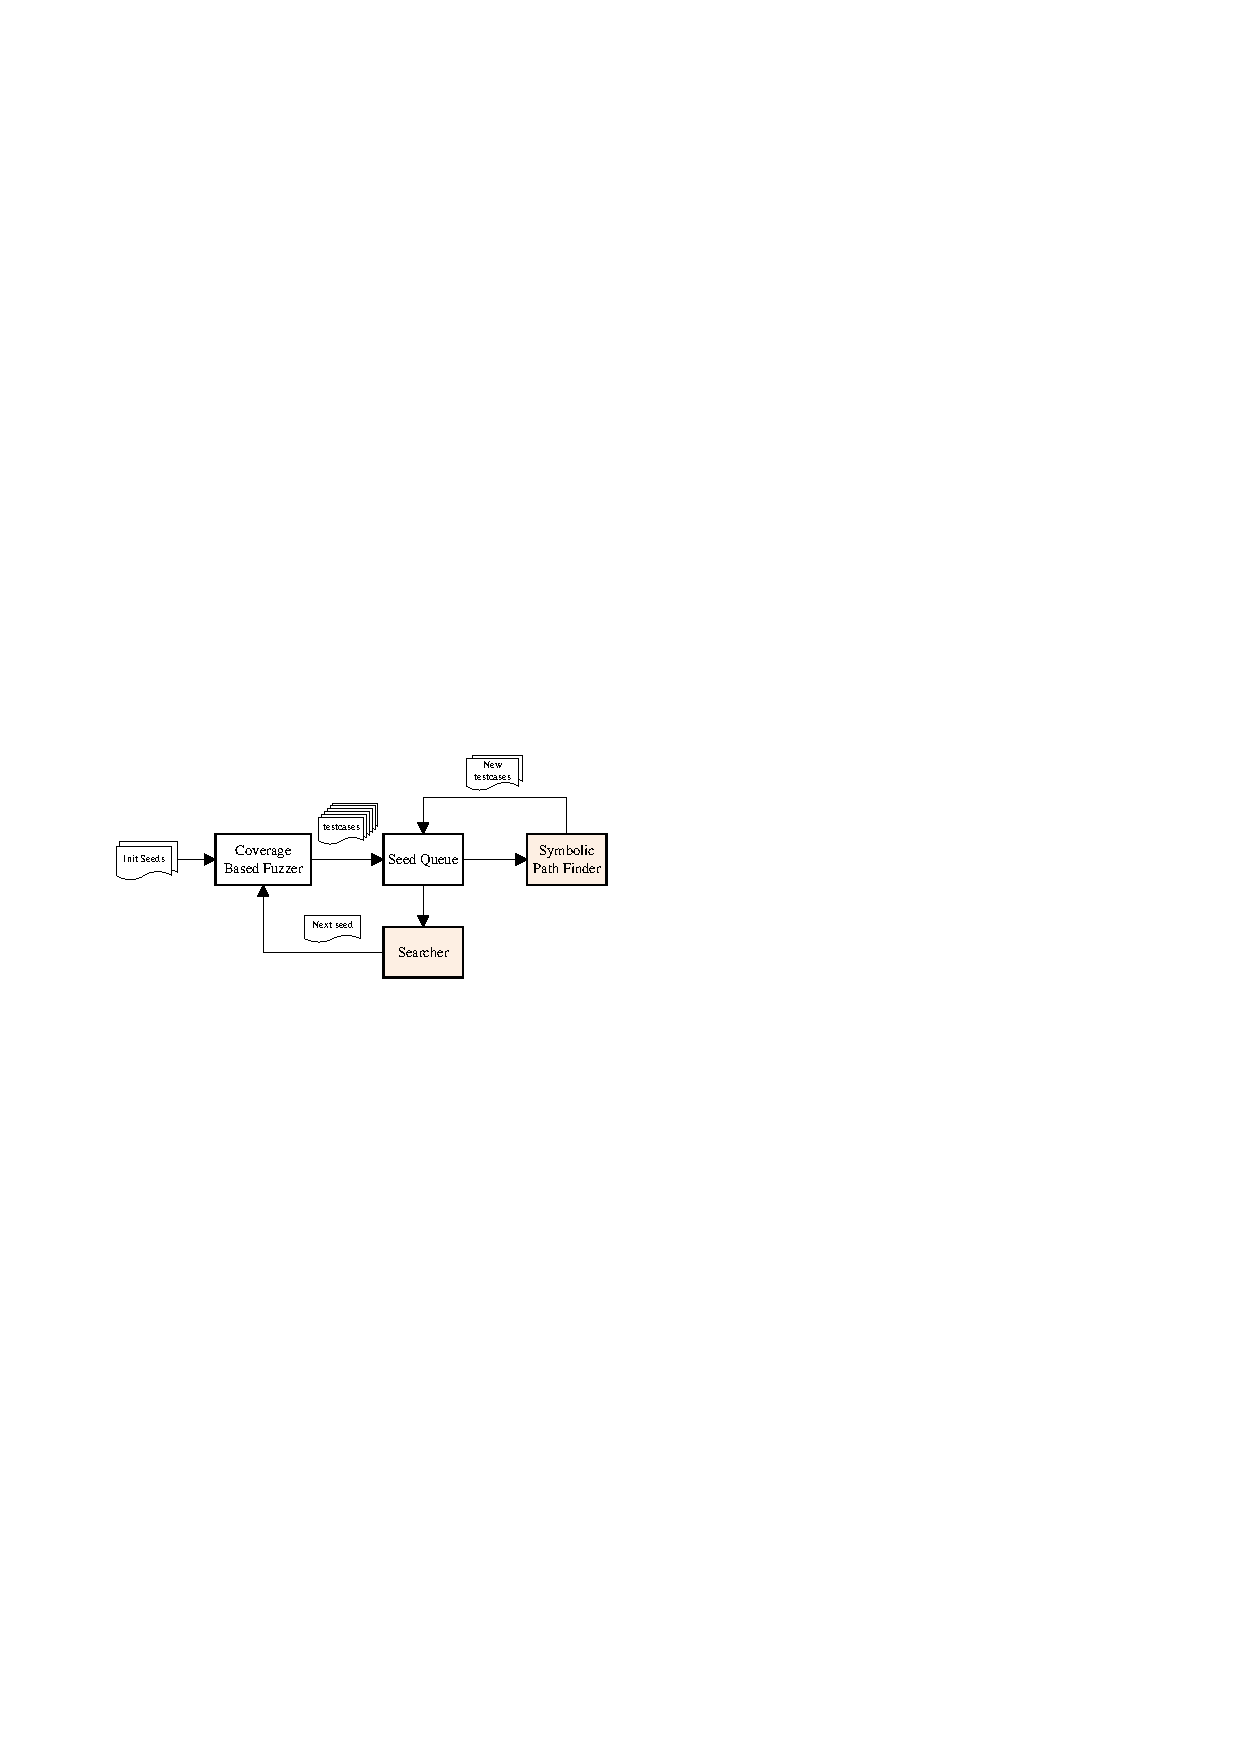
\includegraphics[width=0.7\textwidth]{figures/framework.pdf} 
\caption{High Level Framework.}\label{Framework}
\end{figure}

Figure~\ref{Framework} shows the basic framework of our system. 
From a high-level scope, our method is consisting of two main components, i.e.\emph{SeedSearcher} and \emph{Concolic path finder}. The \emph{SeedSearcher} is designed to select the most promising seed file from the seed queue maintained by the fuzzer based on similarity measurement so that the fuzzer can discover more paths as soon as possible. The \emph{Concolic path finder} component is leveraged to help maximize the code coverage by solving the uncovered first order branch of each seed file in the queue and generate new test cases that can trigger new behaviors of the target program, which will then be added to the seed queue to find more paths by the fuzzer.